%==============================================================================
%  Efficient RAG – Slide thuyết trình BTL IT4772 (Xử lý ngôn ngữ tự nhiên)
%  Beamer 16:9, style HUST đỏ/trắng (theo template slide của nhóm).
%  Biên dịch bằng XeLaTeX (Overleaf: Menu -> Compiler -> XeLaTeX) hoặc `tectonic slides.tex`.
%  Hình trong figures/ do `uv run python scripts/make_figures.py` sinh ra.
%==============================================================================
\documentclass[aspectratio=169,11pt]{beamer}

\usepackage{fontspec}
\setmainfont{texgyreheros}[Extension=.otf, UprightFont=*-regular, BoldFont=*-bold,
  ItalicFont=*-italic, BoldItalicFont=*-bolditalic]
\setsansfont{texgyreheros}[Extension=.otf, UprightFont=*-regular, BoldFont=*-bold,
  ItalicFont=*-italic, BoldItalicFont=*-bolditalic]
\setmonofont{texgyrecursor}[Extension=.otf, UprightFont=*-regular, BoldFont=*-bold,
  ItalicFont=*-italic, BoldItalicFont=*-bolditalic, Scale=MatchLowercase]
\usepackage{microtype}
\usepackage{booktabs}
\usepackage{tabularx}
\usepackage{array}
\usepackage{tikz}
\usetikzlibrary{positioning,arrows.meta,calc,fit,backgrounds}
\graphicspath{{figures/}}

%------------------------------------------------------------------ HUST colours
\definecolor{hustred}{HTML}{A31621}
\definecolor{hustdark}{HTML}{5C0A14}
\definecolor{softgray}{HTML}{8A8A8A}
\definecolor{goodgreen}{HTML}{2A6F5A}

%------------------------------------------------------------------ beamer theme
\usetheme{default}
\useinnertheme{rectangles}
\setbeamercolor{structure}{fg=hustred}
\setbeamercolor{frametitle}{fg=hustred}
\setbeamercolor{title}{fg=hustred}
\setbeamercolor{itemize item}{fg=hustred}
\setbeamercolor{itemize subitem}{fg=hustdark}
\setbeamercolor{enumerate item}{fg=hustred}
\setbeamercolor{block title}{bg=hustred,fg=white}
\setbeamercolor{block body}{bg=hustred!6,fg=black}
\setbeamercolor{alerted text}{fg=hustred}
\setbeamerfont{frametitle}{series=\bfseries}
\setbeamerfont{title}{series=\bfseries}
\setbeamertemplate{navigation symbols}{}
\setbeamertemplate{itemize item}{\small\raise0.2pt\hbox{\textcolor{hustred}{\textbullet}}}
\setbeamertemplate{itemize subitem}{\footnotesize\textcolor{hustdark}{--}}

\setbeamertemplate{frametitle}{%
  \vskip0.5ex%
  \begin{beamercolorbox}[wd=\paperwidth,leftskip=0.9em,rightskip=0.9em]{frametitle}%
    {\usebeamerfont{frametitle}\normalsize\insertframetitle}\par%
    \vskip0.25ex{\color{hustred}\hrule height 0.8pt}%
  \end{beamercolorbox}%
  \vskip0.2ex%
}
\setbeamertemplate{footline}{%
  \hbox{%
    \begin{beamercolorbox}[wd=.5\paperwidth,ht=1.6ex,dp=0.8ex,leftskip=1em]{}%
      {\tiny\color{hustdark}\textbf{Efficient RAG}\;\textcolor{hustred}{\textbar}\;Nén ngữ cảnh \& truy hồi hiệu quả}%
    \end{beamercolorbox}%
    \begin{beamercolorbox}[wd=.5\paperwidth,ht=1.6ex,dp=0.8ex,rightskip=1em]{}%
      \hfill{\tiny\color{hustdark}\insertframenumber\,/\,\inserttotalframenumber}%
    \end{beamercolorbox}%
  }%
  \vskip1.5pt%
}

\newcolumntype{R}{>{\raggedleft\arraybackslash}X}
\newcommand{\best}[1]{\textbf{\color{hustred}#1}}
\newcommand{\todo}[1]{\textcolor{red}{\textbf{[#1]}}}
\makeatletter\newcommand{\inputtable}[1]{\@@input #1 }\makeatother
\newcommand{\takeaway}[1]{{\footnotesize\itshape\color{hustdark}\textbf{Ý chính.} #1\par}}

\title{Efficient RAG: Nén ngữ cảnh và truy hồi hiệu quả}
\date{\small tháng 10 năm 2026}

\begin{document}

%================================================================ 1 — TITLE
{
\setbeamertemplate{footline}{}
\begin{frame}[plain]
  \centering
  {\color{hustred}\rule{\textwidth}{2pt}}\\[0.8ex]
  {\footnotesize\bfseries ĐẠI HỌC BÁCH KHOA HÀ NỘI}\\[0.2ex]
  {\scriptsize\itshape Trường Công nghệ Thông tin và Truyền thông}\\[1.4ex]
  
\includegraphics[height=1.9cm]{hust_logo.png}\\[1.0ex]
  {\Large\bfseries\color{hustred} Efficient RAG}\\[0.4ex]
  {\large\bfseries Nén ngữ cảnh và truy hồi hiệu quả cho hỏi đáp với LLM}\\[0.5ex]
  {\footnotesize Đề tài 13: Efficient LLM/RAG -- Token Compression, Context Compression
  và Efficient Retrieval}\\[1.2ex]
  {\color{hustred}\rule{0.8\textwidth}{0.8pt}}\\[1.2ex]
  {\footnotesize
  \begin{tabular}{@{}r@{\hskip 1.2em}l@{}}
  \textbf{Sinh viên}  & Nguyễn Hoàng Sơn \;(20261127M) \\
                      & Võ Việt Hoàng \;(20251064M) \\
  \textbf{Giảng viên} & Lê Thanh Hương \\
  \textbf{Học phần}   & IT4772 -- Xử lý ngôn ngữ tự nhiên \\
  \end{tabular}}\\[1.0ex]
  {\color{hustred}\rule{\textwidth}{2pt}}
\end{frame}
}

%================================================================ 2 — AGENDA
\begin{frame}{Nội dung}
  \begin{columns}[T]
    \begin{column}{0.5\textwidth}
      \textbf{\color{hustred}I. Bài toán}
      \begin{itemize}\setlength\itemsep{0.2em}
        \item Chi phí ngữ cảnh dài trong RAG
        \item Hiện tượng \emph{lost in the middle}
      \end{itemize}
      \vspace{0.6em}
      \textbf{\color{hustred}II. Phương pháp}
      \begin{itemize}\setlength\itemsep{0.2em}
        \item Benchmark \& giao thức thí nghiệm
        \item 4 nhóm nén cứng · truy hồi hiệu quả
        \item \textbf{Nén mềm ``encode-once''} (đề xuất)
      \end{itemize}
    \end{column}
    \begin{column}{0.5\textwidth}
      \textbf{\color{hustred}III. Kết quả}
      \begin{itemize}\setlength\itemsep{0.2em}
        \item Giữ bằng chứng (không cần LLM)
        \item Độ chính xác -- token -- vị trí
        \item So với số liệu công bố
        \item Nén mềm · truy hồi · CPU vs GPU
      \end{itemize}
      \vspace{0.6em}
      \textbf{\color{hustred}IV. Tổng kết}
      \begin{itemize}\setlength\itemsep{0.2em}
        \item Demo · hạn chế · kết luận
      \end{itemize}
    \end{column}
  \end{columns}
\end{frame}

%================================================================ 3 — PROBLEM
\begin{frame}{Bài toán: ngữ cảnh dài vừa đắt vừa khó dùng}
  \begin{columns}[T]
    \begin{column}{0.52\textwidth}
      \small
      \begin{itemize}\setlength\itemsep{0.4em}
        \item RAG đưa $k$ đoạn văn vào prompt: 20 đoạn NQ $\approx$ \textbf{2.900 token}
          cho một câu hỏi vài chục token.
        \item Chi phí \& độ trễ prefill tăng tuyến tính (attention: bậc hai) theo độ dài.
        \item \textbf{Lost in the middle} (Liu et al., 2024): LLM dùng kém thông tin nằm giữa ngữ cảnh
          -- đường cong chữ U theo vị trí đoạn chứa đáp án.
        \item Hai hướng giảm chi phí:
          \begin{itemize}
            \item \textbf{Nén ngữ cảnh} (Track A): bỏ bớt token/câu/đoạn thừa.
            \item \textbf{Truy hồi hiệu quả} (Track B): lấy đúng đoạn với chỉ mục nhỏ, nhanh.
          \end{itemize}
      \end{itemize}
    \end{column}
    \begin{column}{0.46\textwidth}
      \begin{block}{\small Câu hỏi nghiên cứu}
        \scriptsize
        \textbf{RQ1.} Nén 2--4$\times$ mất bao nhiêu độ chính xác? Có làm phẳng đường cong vị trí?\\[0.3em]
        \textbf{RQ2.} Truy hồi hiệu quả: đánh đổi chất lượng -- tốc độ -- bộ nhớ?\\[0.3em]
        \textbf{RQ3.} Kết luận của bài báo (GPT-3.5) còn đúng với LLM mở 7B?\\[0.3em]
        \textbf{RQ4.} Không có GPU thì có làm được không?\\[0.3em]
        \textbf{RQ5.} Nén mềm ``mã hoá một lần'' (vector) có thay được văn bản?
      \end{block}
    \end{column}
  \end{columns}
\end{frame}

%================================================================ 4 — PIPELINE
\begin{frame}{Hệ thống: truy hồi $\to$ nén $\to$ sinh câu trả lời}
  \centering
  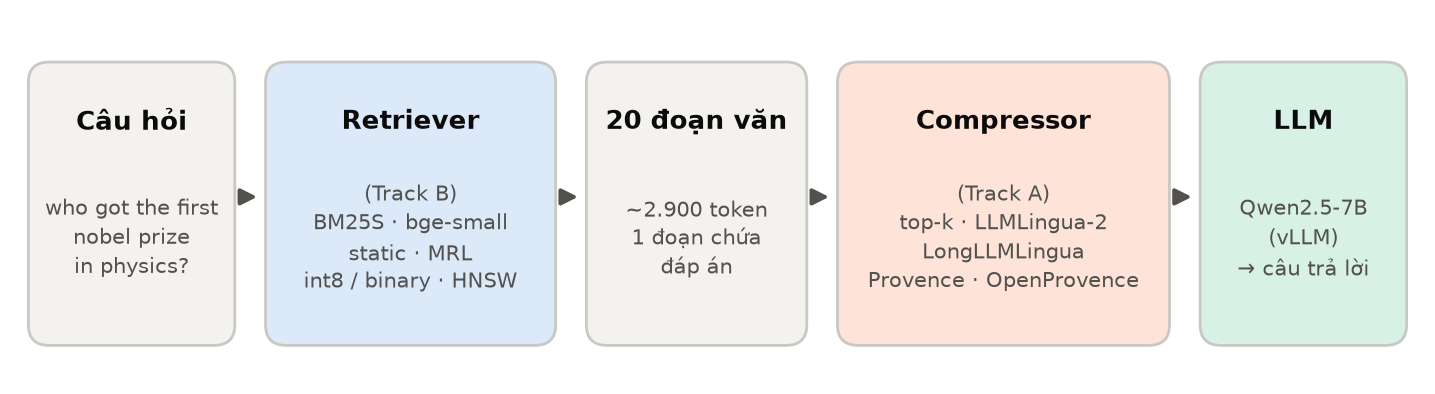
\includegraphics[width=\textwidth]{pipeline.png}
  \vfill
  \begin{columns}[T]
    \begin{column}{0.5\textwidth}
      \scriptsize
      \textbf{\color{hustred}Mã nguồn} gói Python \texttt{effrag} (uv, Python 3.11): mỗi bộ nén
      kế thừa \texttt{Compressor}, mỗi retriever có \texttt{search(queries, k)}; kết quả
      ghi chung một schema (\texttt{summary.csv} + \texttt{.jsonl} từng câu).
    \end{column}
    \begin{column}{0.5\textwidth}
      \scriptsize
      \textbf{\color{hustred}Sinh câu trả lời} Qwen2.5-7B-Instruct-AWQ trên vLLM (GPU 12 GB),
      \texttt{temperature=0}, prompt gốc của Lost in the Middle; cache theo hash prompt
      $\Rightarrow$ chạy lại không tốn chi phí.
    \end{column}
  \end{columns}
\end{frame}

%================================================================ 5 — PROTOCOL
\begin{frame}{Benchmark \& giao thức thí nghiệm}
  \begin{columns}[T]
    \begin{column}{0.5\textwidth}
      \small\textbf{\color{hustred}Dữ liệu}
      {\footnotesize
      \begin{itemize}\setlength\itemsep{0.2em}
        \item NQ-Open 20 đoạn của \emph{Lost in the Middle} (2.655 câu); chọn
          \textbf{500 câu} cố định (seed 42).
        \item Đoạn vàng ở vị trí \textbf{1, 10, 20} -- đúng 3 điểm có số công bố
          của LongLLMLingua / LLMLingua-2.
      \end{itemize}}
      \small\textbf{\color{hustred}Chỉ số}
      {\footnotesize
      \begin{itemize}\setlength\itemsep{0.2em}
        \item Accuracy = đáp án chuẩn hoá nằm trong output (best-subspan EM).
        \item \textbf{Recall bằng chứng}: đáp án còn trong ngữ cảnh sau nén (không cần LLM).
        \item Token (tiktoken \texttt{o200k\_base}), tỉ lệ nén, độ trễ nén.
      \end{itemize}}
    \end{column}
    \begin{column}{0.5\textwidth}
      \begin{block}{\small Thiết kế tiết kiệm tài nguyên}
        \footnotesize
        \begin{itemize}\setlength\itemsep{0.2em}
          \item \textbf{Dry-run} mọi bộ nén trước (miễn phí) $\to$ chỉ gọi LLM cho cấu hình đáng chạy.
          \item Bộ nén theo \emph{từng đoạn} được \textbf{memo hoá} qua các vị trí.
          \item Dùng \textbf{số liệu đã công bố} làm tham chiếu thay vì chạy lại.
          \item Tham chiếu bất biến theo vị trí (closed-book, oracle) chạy 1 lần.
          \item Một job GPU nặng tại một thời điểm; mọi model chạy được trên CPU.
        \end{itemize}
      \end{block}
    \end{column}
  \end{columns}
\end{frame}

%================================================================ 6 — METHODS
\begin{frame}{Các phương pháp nén cứng được so sánh}
  \begingroup\scriptsize
  \renewcommand{\arraystretch}{1.15}
  \begin{tabularx}{\textwidth}{@{}l l X l@{}}
  \toprule
  \textbf{\color{hustred}Mức} & \textbf{\color{hustred}Phương pháp} &
  \textbf{\color{hustred}Ý tưởng} & \textbf{\color{hustred}Nguồn} \\
  \midrule
  Prompt   & Truncate        & cắt đầu ngữ cảnh theo ngân sách token & baseline \\
  Tài liệu & BM25 / Dense / Rerank top-$k$ & chấm điểm đoạn theo câu hỏi, giữ $k$ đoạn, \emph{giữ thứ tự gốc} & bm25s, bge-small, MiniLM CE \\
  Token    & LLMLingua-2     & phân loại giữ/bỏ từng token (XLM-R, chưng cất từ GPT-4) & arXiv 2403.12968 \\
           & LongLLMLingua   & perplexity có điều kiện câu hỏi, ngân sách theo đoạn & arXiv 2310.06839 \\
           & Rerank-10 $\to$ LLMLingua-2 & lọc đoạn rồi nén token & LLMLingua-2 Tab.~4 \\
  Câu      & Provence        & cắt tỉa câu theo câu hỏi, gộp với reranker (DeBERTa) & arXiv 2501.16214 \\
           & OpenProvence    & bản mở, ModernBERT, đa ngôn ngữ & hotchpotch (2025) \\
  \midrule
  Vector   & PISCO           & mỗi đoạn $\to$ 8 vector bộ nhớ (16$\times$), Mistral-7B & arXiv 2501.16075 \\
           & \textbf{Nén mềm encode-once} & \textbf{đề xuất của nhóm} (slide sau) & -- \\
  \bottomrule
  \end{tabularx}\endgroup
  \vfill
  \takeaway{Tỉ lệ mục tiêu 2$\times$ ($\approx$1.450 token) và 4$\times$ ($\approx$730 token) như
  bảng của LongLLMLingua; phương pháp dùng ngưỡng (Provence) báo cáo tỉ lệ thực tế.}
\end{frame}

%================================================================ 7 — SOFT
\begin{frame}{Đề xuất: nén mềm ``encode-once''}
  \begin{columns}[T]
    \begin{column}{0.56\textwidth}
      \centering
      \resizebox{\linewidth}{!}{%
      \begin{tikzpicture}[
        every node/.style={font=\scriptsize},
        box/.style={draw=hustred,fill=hustred!7,rounded corners=2pt,thick,align=center,
                    minimum height=7mm,inner sep=3pt},
        mem/.style={draw=hustdark,fill=hustred!35,minimum width=2.2mm,minimum height=5mm,inner sep=0pt},
        a/.style={-{Stealth[length=2mm]},hustred,thick}]
        \node[box,minimum width=26mm] (d) {Đoạn văn $\le$128 token\\(chạy \textbf{một lần}, offline)};
        \node[box,right=8mm of d,minimum width=20mm] (enc) {Encoder\\LoRA$_{enc}$};
        \draw[a] (d) -- (enc);
        \foreach \i in {0,...,7} \node[mem] (m\i) at ($(enc.east)+(6mm+\i*2.6mm,0)$) {};
        \node[above=0.5mm of m3,xshift=1.3mm,font=\tiny] {8 vector};
        \draw[a] (enc) -- (m0);
        \node[box,below=10mm of enc,minimum width=46mm,xshift=8mm] (dec)
          {Decoder (cùng LLM) + LoRA$_{dec}$\\ câu hỏi + \emph{vector} (+ 1 đoạn text) $\to$ đáp án};
        \draw[a] (m4.south) |- (dec.east);
        \node[box,left=5mm of dec,minimum width=16mm] (q) {Câu hỏi};
        \draw[a] (q) -- (dec);
      \end{tikzpicture}}
      \vspace{0.6em}
      {\scriptsize
      \begin{itemize}\setlength\itemsep{0.15em}
        \item Qwen2.5-1.5B-Instruct, 2 adapter LoRA (r=16) trên \emph{một} model.
        \item 15k câu Tevatron NQ-train (loại câu trùng test), vị trí vàng ngẫu nhiên,
          $k\in\{5,10,20\}$.
        \item \textbf{Biến thể lai}: đoạn top-1 của reranker giữ dạng text
          (tương tự \emph{lightning indexer} của DeepSeek-V3.2: một bộ chấm nhẹ chọn phần
          được xem đầy đủ).
      \end{itemize}}
    \end{column}
    \begin{column}{0.42\textwidth}
      \begin{block}{\small Vì sao?}
        \scriptsize Nén cứng chạy lại \emph{mỗi câu hỏi}. Nén mềm mã hoá kho tài liệu
        \textbf{một lần}; lúc hỏi chỉ đưa 8 vector/đoạn (20 đoạn: 160 vị trí thay vì
        $\approx$2.900 token).
      \end{block}
      \vspace{0.3em}
      \begin{block}{\small Cổng dừng (21/10)}
        \scriptsize 200 câu dev: tiếp tục nếu acc $\ge$ closed-book + 10 điểm và
        $\ge$ 70\% full-text cùng reader; nếu không $\Rightarrow$ báo cáo phân tích thất bại.
      \end{block}
      \vspace{0.3em}
      {\scriptsize\color{hustdark} Đối chứng: PISCO (Naver) huấn luyện trên $>$450k mẫu, 7B;
      nhóm thử ở quy mô BTL (15k mẫu, 1.5B, 1 GPU 12 GB).}
    \end{column}
  \end{columns}
\end{frame}

%================================================================ 8 — RECALL
\begin{frame}{Kết quả 1: bộ nén giữ được bao nhiêu bằng chứng? (không cần LLM)}
  \begin{columns}[T]
    \begin{column}{0.56\textwidth}
      {\scriptsize
      \renewcommand{\arraystretch}{1.12}
      \begin{tabularx}{\textwidth}{@{}X r r r@{}}
      \toprule
      \textbf{\color{hustred}Bộ nén} & \textbf{\color{hustred}Token} &
      \textbf{\color{hustred}Nén} & \textbf{\color{hustred}Recall} \\
      \midrule
      Truncate 730           & 730  & 3,9$\times$ & 100 / 16 / 16$^\dagger$ \\
      BM25 top-5             & 705  & 4,1$\times$ & 53,2 \\
      Dense top-5            & 702  & 4,1$\times$ & 69,0 \\
      Rerank top-5           & 701  & 4,1$\times$ & 79,4 \\
      LLMLingua-2 $r$=0,25   & 827  & 3,5$\times$ & 68,0 \\
      Rerank-10 $\to$ LLMLingua-2 & 743 & 3,9$\times$ & 79,2 \\
      LongLLMLingua 730t$^\ddagger$ & 674 & 4,3$\times$ & 77,5 \\
      \textbf{Provence $\tau$=0,1} & 621 & \textbf{4,6$\times$} & \best{91,6} \\
      \midrule
      Rerank top-10          & 1.425 & 2,0$\times$ & 89,8 \\
      LLMLingua-2 $r$=0,5    & 1.500 & 1,9$\times$ & 88,2 \\
      OpenProvence $\tau$=0,1 & 1.091 & 2,6$\times$ & \best{96,4} \\
      \bottomrule
      \end{tabularx}}\\[0.3em]
      {\tiny $^\dagger$ Truncate: recall ở vị trí 1 / 10 / 20 (cắt mất các đoạn phía sau).
      Các bộ nén khác không phụ thuộc vị trí. $^\ddagger$ n=200, vị trí 10.}
    \end{column}
    \begin{column}{0.42\textwidth}
      \small
      \begin{itemize}\setlength\itemsep{0.4em}
        \item Cùng $\approx$4$\times$, \textbf{Provence giữ 91,6\%} bằng chứng, hơn
          rerank top-5 12 điểm, hơn LLMLingua-2 24 điểm.
        \item Nén mức \emph{câu} theo câu hỏi giữ ngữ nghĩa tốt hơn bỏ token rời rạc.
        \item BM25 trong 20 đoạn đã là hard negative $\Rightarrow$ chỉ 53\%.
      \end{itemize}
      \vfill
      \takeaway{Recall là trần trên của accuracy sau nén, đo được miễn phí trên CPU.}
    \end{column}
  \end{columns}
\end{frame}

%================================================================ 9 — TRADE-OFF
\begin{frame}{Kết quả 2: độ chính xác -- số token (Qwen2.5-7B, 500 câu)}
  \begin{columns}[T]
    \begin{column}{0.6\textwidth}
      \centering
      \IfFileExists{figures/tradeoff.png}{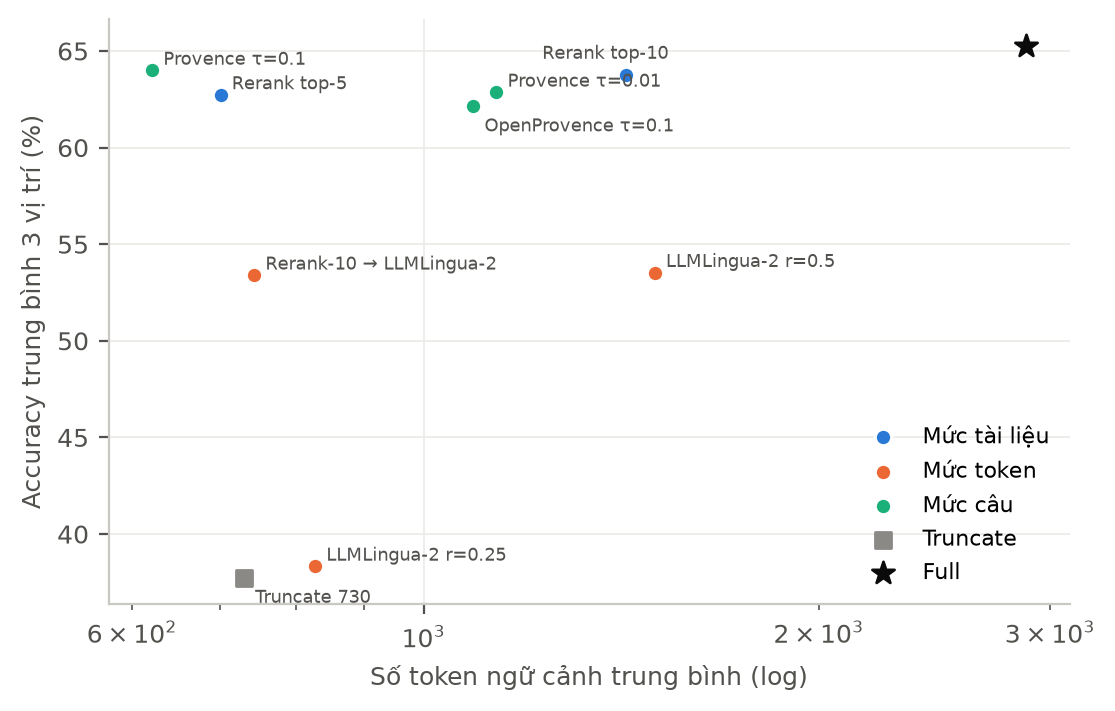
\includegraphics[width=\textwidth]{tradeoff.png}}{\todo{tradeoff.png}}
    \end{column}
    \begin{column}{0.38\textwidth}
      \footnotesize
      \begin{itemize}\setlength\itemsep{0.25em}
        \item Full 20 đoạn: \textbf{65,3}\% (TB 3 vị trí); closed-book 38,8; oracle 92,6.
        \item \textbf{Provence $\tau$=0,1}: 621 token (4,6$\times$), \best{64,0}\% -- không giảm có ý
          nghĩa ở vị trí nào (bootstrap 95\%).
        \item Rerank top-5 (4,1$\times$): 62,7\%; giảm $-6{,}0$ điểm ở vị trí 20.
        \item \textbf{LLMLingua-2} $r$=0,25: 38,3\% $\approx$ closed-book, dù recall còn 68\%.
      \end{itemize}
      \vfill
      \takeaway{Nén mức \emph{câu} theo câu hỏi: 4,6$\times$ ít token, gần như không mất độ chính xác.
      Nén mức \emph{token} làm hỏng văn bản đối với reader 7B.}
    \end{column}
  \end{columns}
\end{frame}

%================================================================ 10 — POSITION
\begin{frame}{Kết quả 3: nén và hiện tượng \emph{lost in the middle}}
  \begin{columns}[T]
    \begin{column}{0.6\textwidth}
      \centering
      \IfFileExists{figures/position_curve.png}{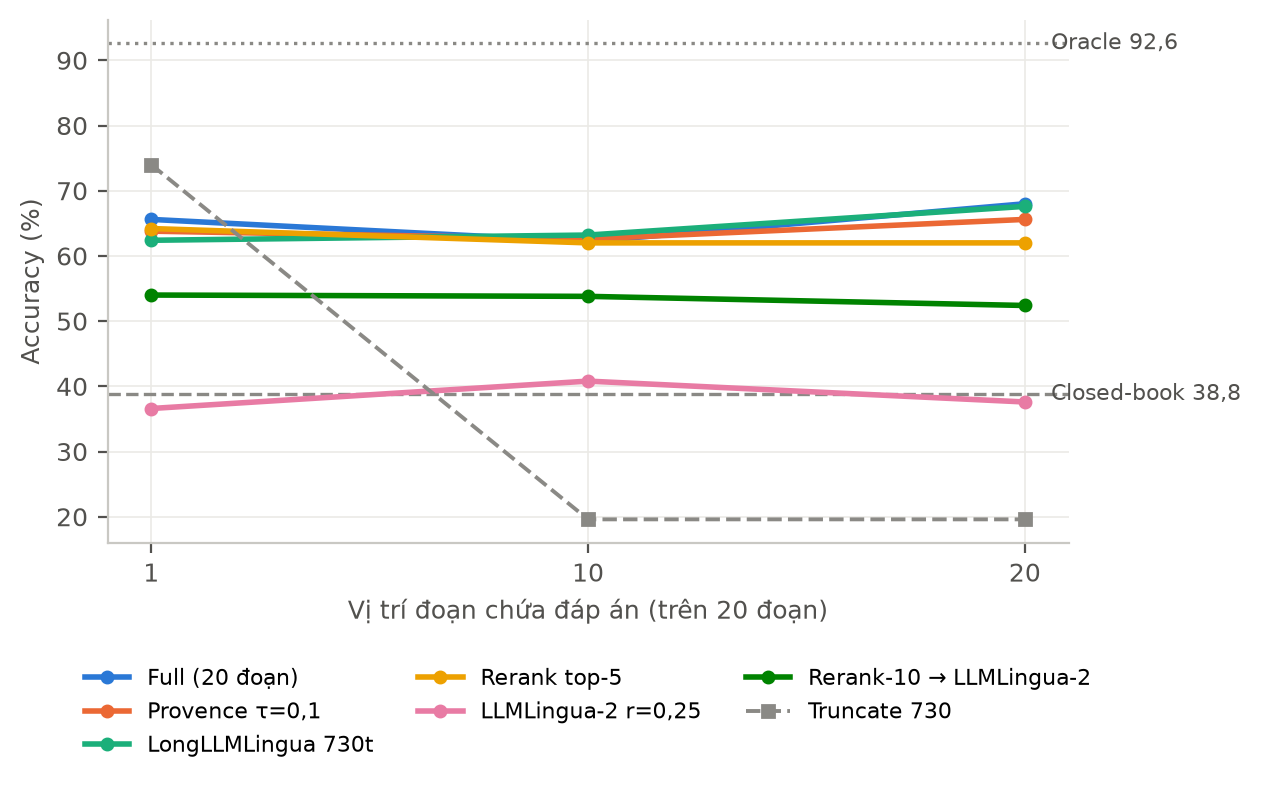
\includegraphics[width=\textwidth]{position_curve.png}}{\todo{position\_curve.png}}
    \end{column}
    \begin{column}{0.38\textwidth}
      \footnotesize
      \begin{itemize}\setlength\itemsep{0.4em}
        \item Full: 65,6 / 62,2 / 68,0 -- gần như \textbf{phẳng} (chênh 5,8 điểm) so với chữ U của
          GPT-3.5: 75,7 / 54,1 / 63,1 (chênh 21,6).
        \item Provence: 63,8 / 62,6 / 65,6 -- song song với Full: không còn nhiều để ``làm phẳng''.
        \item Truncate: 74,0 ở vị trí 1 (\textbf{+8,4}, bớt nhiễu) nhưng 19,6 ở vị trí 10/20.
      \end{itemize}
      \vfill
      \takeaway{Reader hiện đại (ngữ cảnh 32K+) hầu như không còn ``lost in the middle'' ở 3K token.}
    \end{column}
  \end{columns}
\end{frame}

%================================================================ 11 — PUBLISHED
\begin{frame}{Kết quả 4: so với số liệu đã công bố (GPT-3.5-Turbo)}
  \begingroup\scriptsize
  \renewcommand{\arraystretch}{1.12}
  \setlength{\tabcolsep}{3.5pt}
  \begin{tabularx}{\textwidth}{@{}X r r r X r r r@{}}
  \toprule
  \multicolumn{4}{@{}l}{\textbf{\color{hustred}GPT-3.5-Turbo (công bố)}} &
  \multicolumn{4}{l@{}}{\textbf{\color{hustred}Qwen2.5-7B-AWQ (nhóm)}} \\
  & @1 & @10 & @20 & & @1 & @10 & @20 \\
  \midrule
  \inputtable{tables/published.tex}
  \bottomrule
  \end{tabularx}\endgroup\par\vspace{0.3em}
  {\tiny Hàng đầu: accuracy tuyệt đối của ngữ cảnh đầy đủ; các hàng sau: chênh lệch (điểm) so với ngữ
  cảnh đầy đủ của chính hệ đó. LongLLMLingua: so cặp 193 câu.}
  \vfill
  \begin{columns}[T]
    \begin{column}{0.5\textwidth}
      \scriptsize\textbf{\color{goodgreen}Tái lập được}: BM25 $\ll$ Dense; LLMLingua-2 đơn lẻ ở 4$\times$
      sụt nặng ($-$21 đến $-$30 điểm, công bố $-$11 đến $-$27).
    \end{column}
    \begin{column}{0.5\textwidth}
      \scriptsize\textbf{\color{hustred}Không tái lập}: ``nén làm \emph{tăng} accuracy ở giữa''
      (LongLLMLingua $+17{,}1$ $\to$ $+1{,}0$ n.s.) -- vì reader mới không còn lost in the middle.
    \end{column}
  \end{columns}
\end{frame}

%================================================================ 12 — SOFT RESULTS
\begin{frame}{Kết quả 5: nén mềm (PISCO và mô hình của nhóm)}
  \begin{columns}[T]
    \begin{column}{0.6\textwidth}
      \begingroup\scriptsize
      \renewcommand{\arraystretch}{1.08}
      \setlength{\tabcolsep}{3pt}
      \begin{tabularx}{\linewidth}{@{}X r r r r r r@{}}
      \toprule
      Cấu hình & @1 & @10 & @20 & TB & Token & Nén \\
      \midrule
      \inputtable{tables/soft.tex}
      \end{tabularx}\endgroup\par\vspace{0.2em}
      {\tiny Mỗi khối: cùng một reader, chỉ khác ngữ cảnh văn bản / vector. Rerank: chỉ vị trí 10.}
    \end{column}
    \begin{column}{0.37\textwidth}
      \footnotesize
      \begin{itemize}\setlength\itemsep{0.3em}
        \item \textbf{PISCO}: 160 vector thay 2.875 token (18$\times$), TB 48,2\% so với 60,3\% văn bản cùng reader.
        \item Giảm 9 / 10 / 17 điểm ở vị trí 1 / 10 / 20, đều có ý nghĩa; tệ nhất khi đoạn vàng ở cuối.
        \item Rerank-5 $\to$ PISCO: 56,2\% với 40 vector (72$\times$), vẫn kém văn bản rerank-5 6,8 điểm.
        \item \todo{Mô hình của nhóm: mềm / lai}
      \end{itemize}
    \end{column}
  \end{columns}
\end{frame}

%================================================================ 13 — RETRIEVAL
\begin{frame}{Kết quả 6: truy hồi hiệu quả (corpus gộp 50,7k đoạn, 500 câu)}
  \begin{columns}[T]
    \begin{column}{0.55\textwidth}
      \centering
      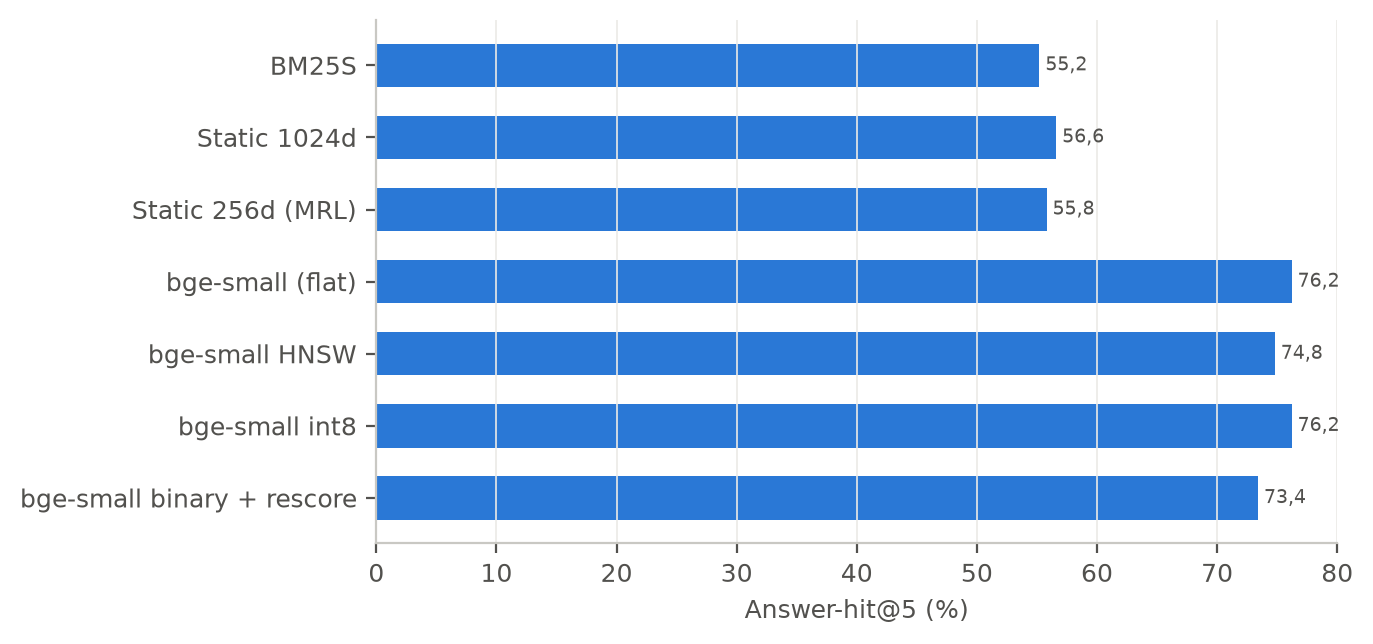
\includegraphics[width=\textwidth]{retrieval_hit5.png}
    \end{column}
    \begin{column}{0.43\textwidth}
      {\scriptsize
      \renewcommand{\arraystretch}{1.12}
      \begin{tabularx}{\textwidth}{@{}X r r@{}}
      \toprule
      \textbf{\color{hustred}Hệ thống} & \textbf{\color{hustred}hit@5} & \textbf{\color{hustred}Chỉ mục} \\
      \midrule
      BM25S                 & 55,2 & -- \\
      Static embedding 256d & 55,8 & 49,5 MB \\
      bge-small fp32        & 76,2 & 74,3 MB \\
      bge-small \textbf{int8} & \best{76,2} & \textbf{18,6 MB} \\
      binary + rescore      & 73,4 & \textbf{2,3 MB} \\
      \bottomrule
      \end{tabularx}}
      \vspace{0.6em}
      \takeaway{Lượng tử hoá int8 giảm 4$\times$ bộ nhớ không mất điểm; binary + rescore
      giảm 32$\times$ chỉ mất 2,8 điểm.}
    \end{column}
  \end{columns}
\end{frame}

%================================================================ 14 — CPU
\begin{frame}{Kết quả 7: không có GPU thì sao?}
  \begin{columns}[T]
    \begin{column}{0.55\textwidth}
      \begingroup\scriptsize
      \renewcommand{\arraystretch}{1.1}
      \begin{tabularx}{\linewidth}{@{}X r r r@{}}
      \toprule
      Bộ nén & GPU & CPU & $\times$ \\
      \midrule
      \inputtable{tables/latency.tex}
      \bottomrule
      \end{tabularx}\endgroup\par\vspace{0.2em}
      {\tiny Trung vị ms/câu, 20 câu, không tính LLM. RTX 4070 SUPER vs i5-14600K 8 luồng.}
    \end{column}
    \begin{column}{0.42\textwidth}
      \footnotesize
      \begin{itemize}\setlength\itemsep{0.3em}
        \item \textbf{Mức tài liệu} $<$ 0,4 s trên CPU: dùng tương tác được.
        \item \textbf{Mức câu} chậm 21--25$\times$: Provence 4,9 s, OpenProvence 1,6 s.
        \item \textbf{Mức token} 13--15 s và accuracy kém hơn $\Rightarrow$ không nên dùng khi thiếu GPU.
        \item Reader qua API: Provence giảm \textbf{78\%} token đầu vào, $-$1,3 điểm (n.s.).
      \end{itemize}
    \end{column}
  \end{columns}
  \vfill
  \takeaway{Không có GPU vẫn chạy được: rerank top-5 (0,2 s) hoặc Provence (4,9 s) trên CPU + reader qua API.}
\end{frame}

%================================================================ 15 — DEMO
\begin{frame}{Demo (Gradio): so sánh bộ nén trên cùng một câu hỏi}
  \begin{columns}[T]
    \begin{column}{0.52\textwidth}
      \centering
      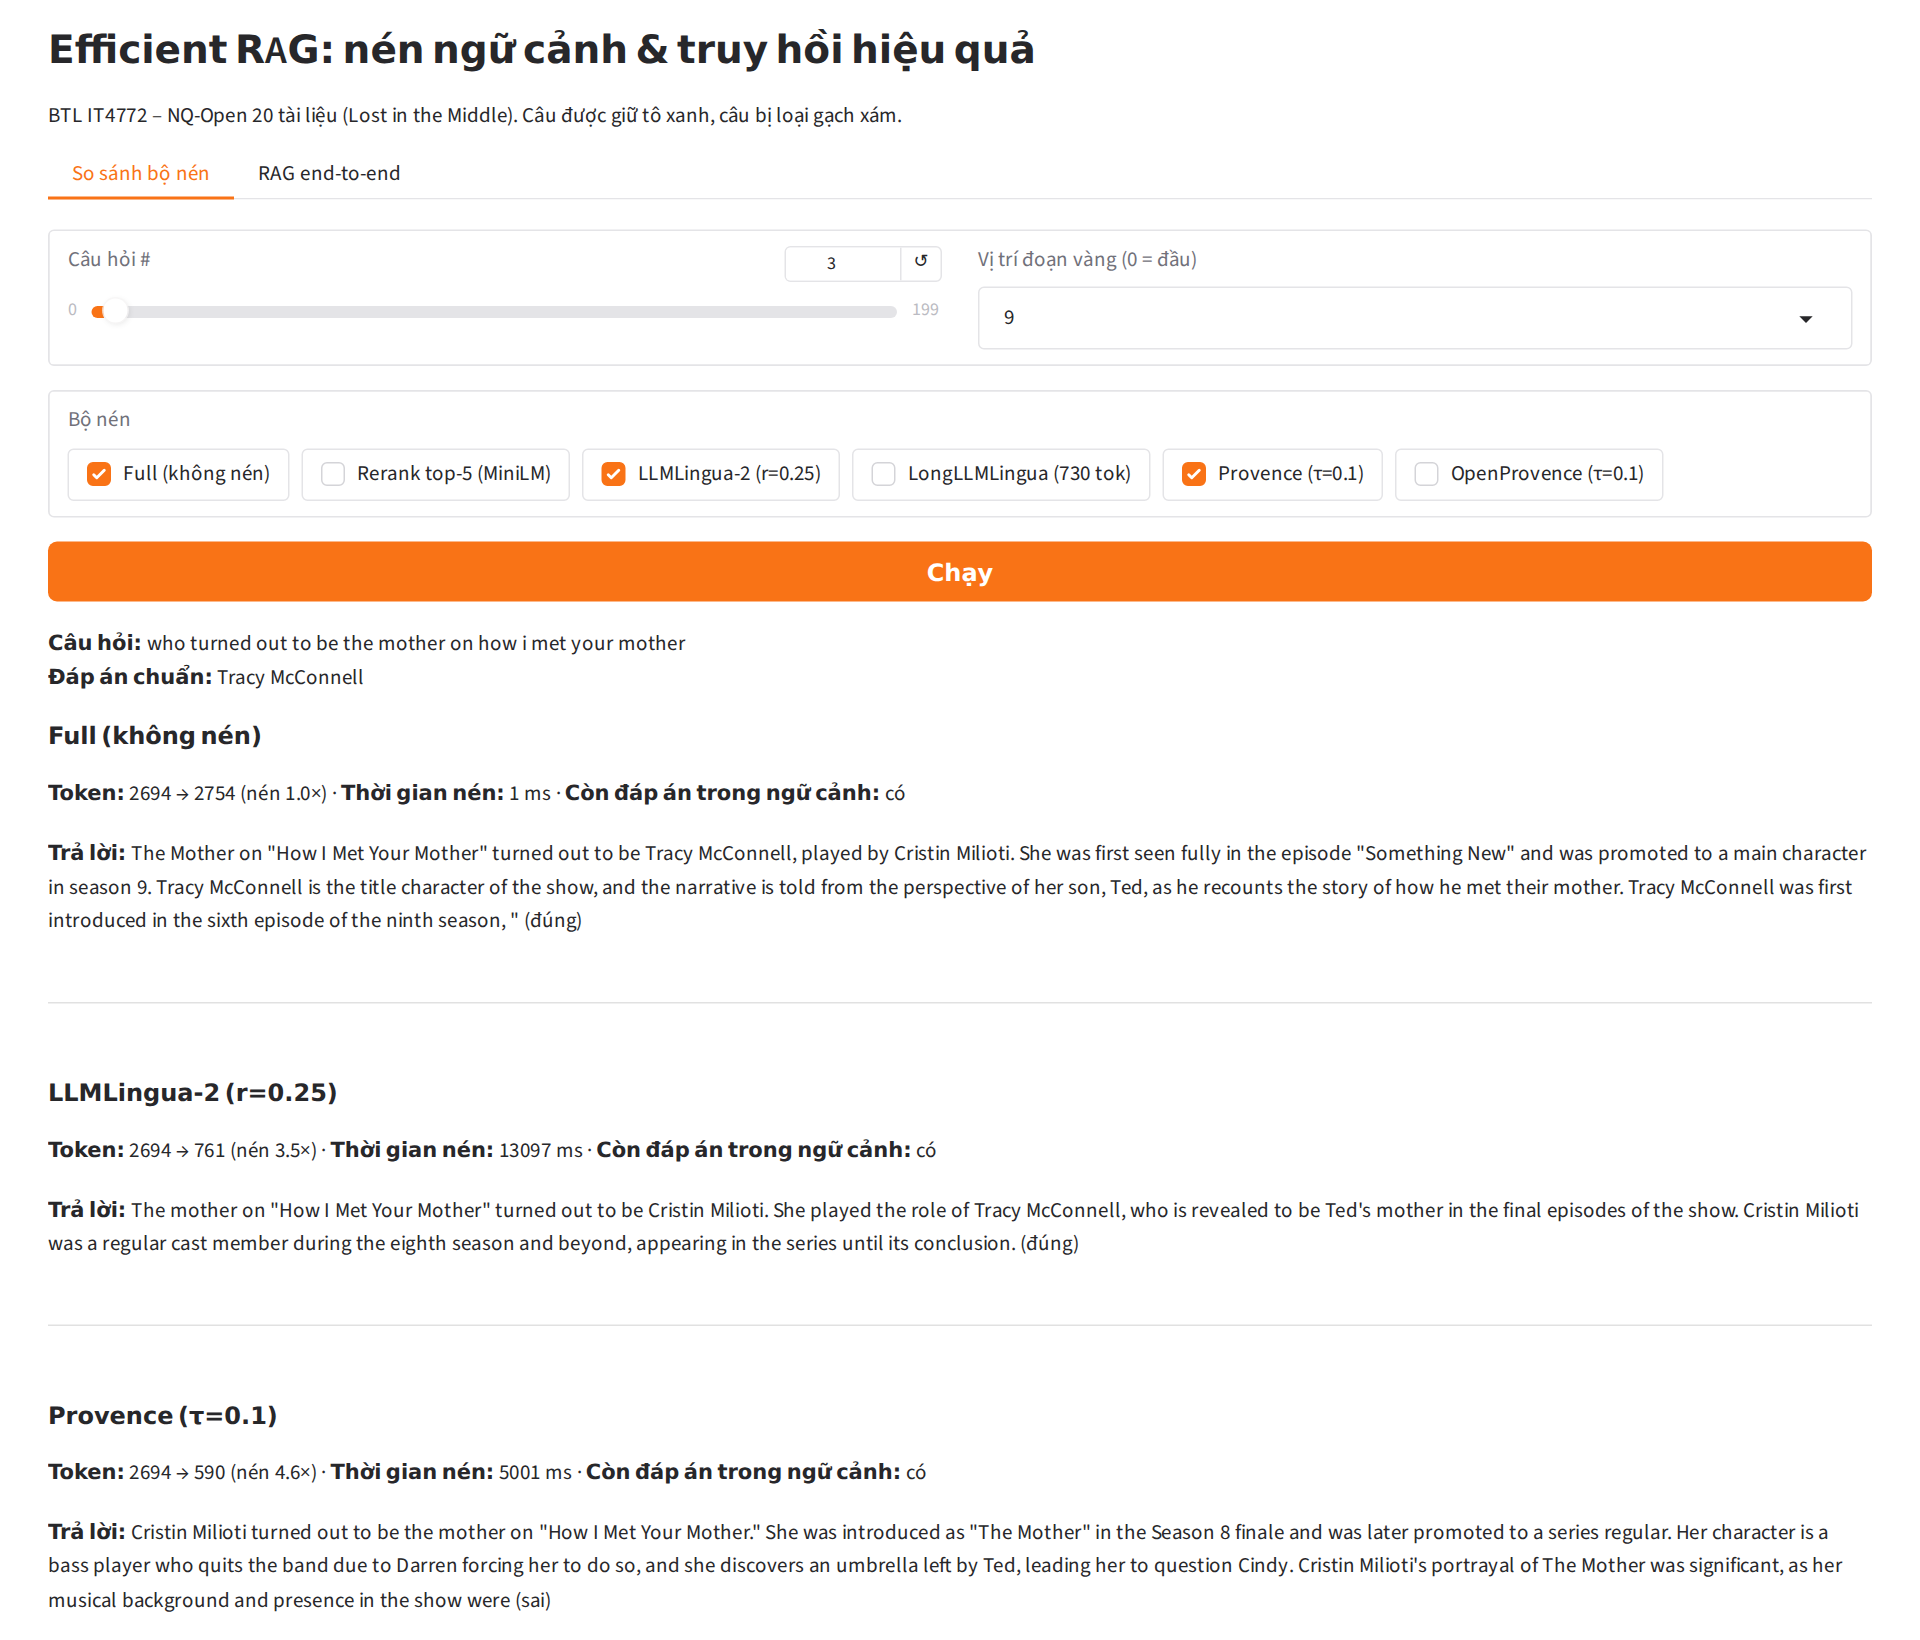
\includegraphics[width=\textwidth]{demo.png}
    \end{column}
    \begin{column}{0.46\textwidth}
      \centering
      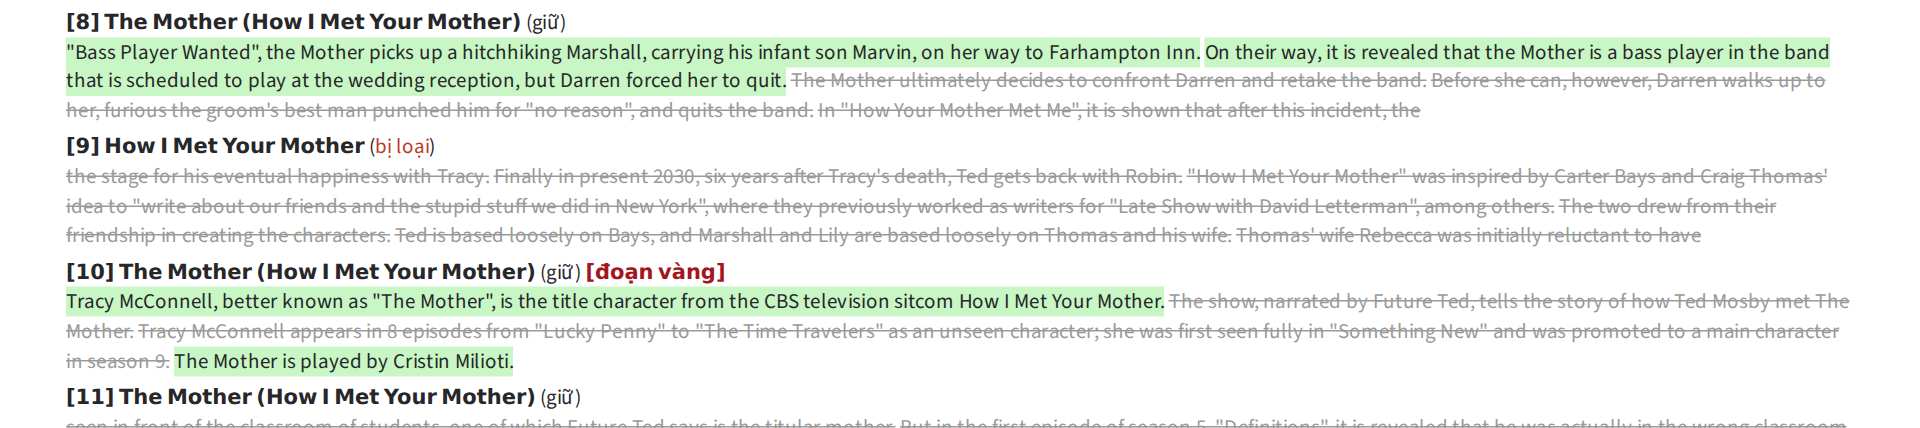
\includegraphics[width=\textwidth]{demo_context.png}\\[0.6em]
      {\scriptsize
      \begin{itemize}\setlength\itemsep{0.2em}
        \item Token trước/sau, thời gian nén, đáp án còn trong ngữ cảnh, câu trả lời LLM.
        \item Câu được giữ tô xanh, câu bị loại gạch ngang; đoạn vàng được đánh dấu.
        \item Tab 2: câu hỏi tự do $\to$ BM25S/bge-small (50,7k đoạn) $\to$ nén $\to$ LLM.
        \item Chạy hoàn toàn trên CPU; không có LLM vẫn xem được phần nén.
      \end{itemize}}
    \end{column}
  \end{columns}
\end{frame}

%================================================================ 16 — CONCLUSION
\begin{frame}{Hạn chế \& kết luận}
  \begin{columns}[T]
    \begin{column}{0.5\textwidth}
      \small\textbf{\color{hustred}Hạn chế}
      {\footnotesize
      \begin{itemize}\setlength\itemsep{0.3em}
        \item Một LLM 7B lượng tử hoá, một tập (NQ); số công bố dùng GPT-3.5 đã ngừng.
        \item 500 câu, 3 vị trí; LongLLMLingua chỉ 200 câu ở vị trí 10.
        \item Nén mềm huấn luyện ở quy mô nhỏ (15k mẫu, 1.5B).
      \end{itemize}}
    \end{column}
    \begin{column}{0.5\textwidth}
      \small\textbf{\color{hustred}Kết luận}
      {\footnotesize
      \begin{itemize}\setlength\itemsep{0.3em}
        \item \textbf{Chọn câu > chọn tài liệu > xoá token}: Provence 4,6$\times$, $-$1,3 điểm (n.s.);
        LLMLingua-2 4$\times$ về mức closed-book.
        \item Reader mới gần như hết \emph{lost in the middle} $\Rightarrow$ lợi ích ``nén làm tăng
        accuracy'' của GPT-3.5 không còn.
        \item Không GPU vẫn làm được: nén trên CPU + reader qua API; dense nhỏ int8 cho truy hồi.
        % TODO(T18): one bullet on soft compression
      \end{itemize}}
    \end{column}
  \end{columns}
  \vspace{0.8em}
  \begin{center}
    {\color{hustred}\rule{0.7\textwidth}{1pt}}\\[0.7ex]
    {\Large\bfseries\color{hustred} Cảm ơn thầy cô và các bạn đã lắng nghe!}\\[0.4ex]
    {\color{hustred}\rule{0.7\textwidth}{1pt}}
  \end{center}
\end{frame}

\end{document}
